% Chantier 95 -- Masked Mandates -- supplementary material (full definitions and proofs), version 2.1.
% Build: pdflatex supplement && bibtex supplement && pdflatex supplement && pdflatex supplement
\documentclass[10pt]{article}
\usepackage[margin=2.2cm]{geometry}
\usepackage{amsmath,amssymb,amsthm}
\usepackage{enumitem}
\usepackage{cite}
\usepackage{url}
\usepackage{booktabs,array,graphicx}
\usepackage{tikz}
\usepackage{hyperref}
\hypersetup{hidelinks}
\newtheorem{definition}{Definition}
\newtheorem{theorem}{Theorem}
\newtheorem{lemma}{Lemma}
\newtheorem{assumption}{Assumption}
\newtheorem{remark}{Remark}
\newcommand{\sys}{\textsc{Masked Mandates}}
\newcommand{\Allow}{\mathsf{Allow}}
\newcommand{\Live}{\mathsf{Live}}
\newcommand{\Adv}{\mathsf{Adv}}
\newcommand{\negl}{\mathsf{negl}}
\newcommand{\ctx}{\mathsf{ctx}}
\newcommand{\nym}{\mathit{nym}}
\newcommand{\Zq}{\mathbb{Z}_q}
\newcommand{\G}{\mathbb{G}_1}
\newcommand{\Iss}{\mathcal{I}}
\newcommand{\Esc}{\mathcal{E}}
\newcommand{\Ext}{\mathsf{Ext}}
\newcommand{\Sim}{\mathsf{Sim}}
\newcommand{\PoK}{\mathsf{PoK}}
\newcommand{\Lset}{\mathcal{L}}
\newcommand{\Rset}{\mathcal{R}}
\newcommand{\Log}{\mathsf{Log}}

\title{Masked Mandates: Unlinkable, Attenuable and Accountable Delegation for LLM Agents\\[4pt]\large Supplementary material: definitions and security proofs}
\author{Yulliwas Ameur, Samia Bouzefrane, Soumya Banerjee}
\date{}

% generated by gen_tex_v21.py from results/ -- do not edit
\newcommand{\AblBbsPres}{4}
\newcommand{\AblDyAdd}{165}
\newcommand{\AblHideCost}{0.5}
\newcommand{\AblNmAdd}{58}
\newcommand{\AblRangeAdd}{163}
\newcommand{\AblRevAdd}{165}
\newcommand{\AblRevPres}{168}
\newcommand{\BenchN}{100}
\newcommand{\CampSpread}{0.5\,\%}
\newcommand{\CoalFiveName}{51\,\%}
\newcommand{\CpuMac}{Apple M5 Pro}
\newcommand{\CpuZen}{AMD EPYC 9534}
\newcommand{\DecJoinCandDay}{5.5}
\newcommand{\DecJoinCandDayTenK}{44.8}
\newcommand{\DecJoinCandHour}{1.2}
\newcommand{\DecJoinCandHourTenK}{3.7}
\newcommand{\DecJoinPrecDay}{44\,\%}
\newcommand{\DecJoinPrecDayTenK}{23\,\%}
\newcommand{\DecJoinPrecHour}{83\,\%}
\newcommand{\DecJoinPrecHourTenK}{50\,\%}
\newcommand{\DelIssuerMs}{423}
\newcommand{\DelMsgHiS}{5.23}
\newcommand{\DelMsgLoMs}{1{,}293}
\newcommand{\DelParentS}{2.28}
\newcommand{\DelegLatMedS}{2.44}
\newcommand{\DepthPresMax}{390}
\newcommand{\DepthPresMin}{390}
\newcommand{\EBaseMaxHttp}{6.4}
\newcommand{\ECalls}{200}
\newcommand{\EChalHttp}{3.6}
\newcommand{\EFourCalls}{83{,}764}
\newcommand{\EFourCanonCalls}{83{,}764}
\newcommand{\EFourCfgs}{6}
\newcommand{\EFourCpu}{Intel~Xeon Platinum 8462Y+}
\newcommand{\EFourDelegS}{2.46}
\newcommand{\EFourDelegShareMax}{22\,\%}
\newcommand{\EFourDeltaDelayS}{1.2}
\newcommand{\EFourDeltaDelaySparseS}{1.2}
\newcommand{\EFourDeltaRej}{0}
\newcommand{\EFourDwLlmHonest}{2{,}147}
\newcommand{\EFourDwLlmSent}{629}
\newcommand{\EFourDwQuotaSent}{48}
\newcommand{\EFourDwRevSent}{48}
\newcommand{\EFourDwSent}{96}
\newcommand{\EFourEqAll}{14}
\newcommand{\EFourEqPairs}{15}
\newcommand{\EFourEqTsev}{12}
\newcommand{\EFourHonestCalls}{37{,}795}
\newcommand{\EFourIpcMs}{0.14}
\newcommand{\EFourJwtShareMax}{0.5\,\%}
\newcommand{\EFourJwtSlowMax}{1.00}
\newcommand{\EFourLatMed}{120}
\newcommand{\EFourLlmFixSuccMax}{95}
\newcommand{\EFourLlmFixSuccMin}{89}
\newcommand{\EFourMMEq}{5}
\newcommand{\EFourMMEqTsev}{4}
\newcommand{\EFourMMMaxDiff}{0.6}
\newcommand{\EFourMMMaxDiffTsev}{0.9}
\newcommand{\EFourMarginPP}{5}
\newcommand{\EFourMinHolm}{1.00}
\newcommand{\EFourMinP}{0.12}
\newcommand{\EFourModels}{5}
\newcommand{\EFourMtPres}{121}
\newcommand{\EFourMtVer}{63}
\newcommand{\EFourNTests}{30}
\newcommand{\EFourNoneSafeMax}{0.7}
\newcommand{\EFourNotEqTsev}{Granite-3.3-8B MM+escrow, gpt-oss-20b MM, gpt-oss-20b MM+escrow}
\newcommand{\EFourNudgeMax}{37}
\newcommand{\EFourNudgeMin}{0}
\newcommand{\EFourOrWzeroRej}{17\,\%}
\newcommand{\EFourPresMs}{353}
\newcommand{\EFourProbeCases}{63}
\newcommand{\EFourQuotaAtt}{3{,}735}
\newcommand{\EFourQuotaMax}{99}
\newcommand{\EFourQuotaMin}{2.1}
\newcommand{\EFourQuotaNone}{1{,}454}
\newcommand{\EFourRepDetModel}{Qwen2.5-72B}
\newcommand{\EFourRepMax}{7}
\newcommand{\EFourRepPP}{10}
\newcommand{\EFourRepPairs}{72}
\newcommand{\EFourRetryCalls}{696}
\newcommand{\EFourRetryDelayMs}{245}
\newcommand{\EFourRetryN}{192}
\newcommand{\EFourRetryOk}{192}
\newcommand{\EFourRetryRej}{0}
\newcommand{\EFourRevAtt}{1{,}954}
\newcommand{\EFourRevNone}{926}
\newcommand{\EFourRuns}{14{,}400}
\newcommand{\EFourSafeMax}{100}
\newcommand{\EFourSafeMin}{17}
\newcommand{\EFourSdk}{1.30.0}
\newcommand{\EFourShBaseMax}{94}
\newcommand{\EFourShBaseMin}{88}
\newcommand{\EFourShDelayTwoS}{4.2}
\newcommand{\EFourShDelayZeroMs}{239}
\newcommand{\EFourShEvery}{2}
\newcommand{\EFourShRejMax}{19\,\%}
\newcommand{\EFourShRejMin}{17\,\%}
\newcommand{\EFourShSuccTwoMax}{96}
\newcommand{\EFourShSuccTwoMin}{88}
\newcommand{\EFourShSuccZeroMax}{65}
\newcommand{\EFourShSuccZeroMin}{52}
\newcommand{\EFourShTasks}{120}
\newcommand{\EFourShareMax}{59\,\%}
\newcommand{\EFourShareMin}{35\,\%}
\newcommand{\EFourSlowMax}{2.32}
\newcommand{\EFourSlowMin}{1.49}
\newcommand{\EFourSlowNoLatMax}{3.12}
\newcommand{\EFourTasks}{120}
\newcommand{\EFourUnitsAll}{360}
\newcommand{\EFourUnitsTsev}{216}
\newcommand{\EFourVerMs}{95}
\newcommand{\EFourVllm}{0.33.0}
\newcommand{\EFourWtwoDelayS}{4.2}
\newcommand{\EFourWtwoDelaySparseS}{120}
\newcommand{\EMMBytes}{18{,}115}
\newcommand{\EMMDelegS}{4.01}
\newcommand{\EMMPrep}{291}
\newcommand{\EMMTotalDelay}{422}
\newcommand{\EMMTotalHi}{379}
\newcommand{\EMMTotalHttp}{377}
\newcommand{\EMMTotalLo}{376}
\newcommand{\EMMVer}{78}
\newcommand{\EMcpSdk}{1.30.0}
\newcommand{\EPy}{3.13.16}
\newcommand{\ERuns}{3}
\newcommand{\EStatelessAdd}{26}
\newcommand{\EStatelessAddJwt}{25}
\newcommand{\EWarm}{15}
\newcommand{\EscExtraB}{500}
\newcommand{\EtoeNoneHttp}{3.0}
\newcommand{\GapMedS}{0.78}
\newcommand{\GapModels}{5}
\newcommand{\GapN}{8{,}527}
\newcommand{\GapNinetyNineS}{5.6}
\newcommand{\GapNinetyS}{2.1}
\newcommand{\GapRows}{1{,}776}
\newcommand{\GapSource}{E4 v2.1 \sys{} runs}
\newcommand{\GitCommit}{96a694d14ca4}
\newcommand{\IssExactA}{71\,\%}
\newcommand{\IssExactAPdOne}{71\,\%}
\newcommand{\IssExactAPdOneTenK}{19\,\%}
\newcommand{\IssExactATenK}{19\,\%}
\newcommand{\IssExactI}{75\,\%}
\newcommand{\IssExactIPdOne}{87\,\%}
\newcommand{\IssExactIPdOneTenK}{33\,\%}
\newcommand{\IssExactITenK}{22\,\%}
\newcommand{\IssLagMedS}{1.06}
\newcommand{\IssLagNinetyNineS}{1.75}
\newcommand{\IssNDeleg}{556}
\newcommand{\IssNameInc}{1.1}
\newcommand{\IssNameIncHi}{1.4}
\newcommand{\IssNameIncHiPdOne}{5.2}
\newcommand{\IssNameIncHiPdOneTenK}{8.2}
\newcommand{\IssNameIncHiTenK}{1.7}
\newcommand{\IssNameIncLo}{0.9}
\newcommand{\IssNameIncLoPdOne}{3.7}
\newcommand{\IssNameIncLoPdOneTenK}{3.9}
\newcommand{\IssNameIncLoTenK}{0.8}
\newcommand{\IssNameIncPdOne}{4.3}
\newcommand{\IssNameIncPdOneTenK}{5.7}
\newcommand{\IssNameIncTenK}{1.2}
\newcommand{\IssNameWith}{70\,\%}
\newcommand{\IssNameWithPdOne}{73\,\%}
\newcommand{\IssNameWithPdOneTenK}{47\,\%}
\newcommand{\IssNameWithTenK}{43\,\%}
\newcommand{\IssPDeleg}{31\,\%}
\newcommand{\IssSessInc}{1.1}
\newcommand{\IssSessIncLoadHi}{0.0}
\newcommand{\IssSessIncLoadHiRate}{104}
\newcommand{\IssSessIncPdOne}{3.7}
\newcommand{\IssSessIncPdOneTenK}{4.8}
\newcommand{\IssSessIncTenK}{1.0}
\newcommand{\JitDSixHundred}{0.1\,\%}
\newcommand{\JitDSixty}{0.1\,\%}
\newcommand{\JitDTen}{0.0\,\%}
\newcommand{\JitNameSixHundred}{34\,\%}
\newcommand{\JitNameSixty}{37\,\%}
\newcommand{\JitNameTen}{50\,\%}
\newcommand{\LinkCalls}{179{,}802}
\newcommand{\LinkDayReid}{13\,\%}
\newcommand{\LinkDays}{30}
\newcommand{\LinkMMMinReid}{0.5\,\%}
\newcommand{\LinkMMMinSensMax}{2.0\,\%}
\newcommand{\LinkMMReid}{6.7\,\%}
\newcommand{\LinkMMReidHi}{10\,\%}
\newcommand{\LinkMMReidLo}{3.3\,\%}
\newcommand{\LinkMMUpper}{43\,\%}
\newcommand{\LinkPertoolReid}{94\,\%}
\newcommand{\LinkPtejOracle}{83\,\%}
\newcommand{\LinkPtejReid}{24\,\%}
\newcommand{\LinkSeeds}{5}
\newcommand{\LinkTools}{50}
\newcommand{\LoadRateMax}{104}
\newcommand{\LoadRateMin}{0.35}
\newcommand{\LoadUsersMax}{100{,}000}
\newcommand{\MsgBMax}{14{,}688}
\newcommand{\MsgBMin}{13{,}152}
\newcommand{\MsgHi}{65}
\newcommand{\MsgLo}{17}
\newcommand{\MsgPresMax}{392}
\newcommand{\MsgPresMin}{390}
\newcommand{\NAttMDel}{7}
\newcommand{\NAttMP}{13}
\newcommand{\NAttMPReach}{12}
\newcommand{\NAttProver}{12}
\newcommand{\NAttReach}{84}
\newcommand{\NAttacks}{96}
\newcommand{\NBitFlips}{2{,}000}
\newcommand{\NChecks}{37}
\newcommand{\NMsgs}{29}
\newcommand{\NameDay}{70\,\%}
\newcommand{\NameDecDay}{20\,\%}
\newcommand{\NameDecDayAdapt}{34\,\%}
\newcommand{\NameDecDayAdaptHi}{46\,\%}
\newcommand{\NameDecDayAdaptLo}{25\,\%}
\newcommand{\NameDecDayAdaptSess}{21\,\%}
\newcommand{\NameDecDayAdaptSessTenK}{15\,\%}
\newcommand{\NameDecDayAdaptTenK}{18\,\%}
\newcommand{\NameDecDayAdaptTenKHi}{22\,\%}
\newcommand{\NameDecDayAdaptTenKLo}{14\,\%}
\newcommand{\NameDecDayEvery}{61\,\%}
\newcommand{\NameDecDayEveryHi}{72\,\%}
\newcommand{\NameDecDayEveryLo}{50\,\%}
\newcommand{\NameDecDayFree}{17\,\%}
\newcommand{\NameDecDayFreeHi}{23\,\%}
\newcommand{\NameDecDayFreeLo}{11\,\%}
\newcommand{\NameDecDayFreeSess}{13\,\%}
\newcommand{\NameDecDayFreeSessTenK}{12\,\%}
\newcommand{\NameDecDayFreeTenK}{13\,\%}
\newcommand{\NameDecDayFreeTenKHi}{16\,\%}
\newcommand{\NameDecDayFreeTenKLo}{9.2\,\%}
\newcommand{\NameDecDayFreeTools}{20\,\%}
\newcommand{\NameDecDayFreeToolsHi}{25\,\%}
\newcommand{\NameDecDayFreeToolsLo}{14\,\%}
\newcommand{\NameDecDayFreeToolsTenK}{15\,\%}
\newcommand{\NameDecDayFreeToolsTenKHi}{19\,\%}
\newcommand{\NameDecDayFreeToolsTenKLo}{11\,\%}
\newcommand{\NameDecDayHi}{25\,\%}
\newcommand{\NameDecDayLo}{14\,\%}
\newcommand{\NameDecDayMin}{15\,\%}
\newcommand{\NameDecDaySess}{14\,\%}
\newcommand{\NameDecDayTenK}{15\,\%}
\newcommand{\NameDecDayTenKHi}{19\,\%}
\newcommand{\NameDecDayTenKLo}{11\,\%}
\newcommand{\NameDecHour}{22\,\%}
\newcommand{\NameDecHourAdapt}{44\,\%}
\newcommand{\NameDecHourAdaptHi}{60\,\%}
\newcommand{\NameDecHourAdaptLo}{30\,\%}
\newcommand{\NameDecHourAdaptSess}{29\,\%}
\newcommand{\NameDecHourAdaptSessTenK}{20\,\%}
\newcommand{\NameDecHourAdaptTenK}{24\,\%}
\newcommand{\NameDecHourAdaptTenKHi}{32\,\%}
\newcommand{\NameDecHourAdaptTenKLo}{17\,\%}
\newcommand{\NameDecHourEvery}{61\,\%}
\newcommand{\NameDecHourEveryHi}{72\,\%}
\newcommand{\NameDecHourEveryLo}{51\,\%}
\newcommand{\NameDecHourFree}{20\,\%}
\newcommand{\NameDecHourFreeHi}{25\,\%}
\newcommand{\NameDecHourFreeLo}{14\,\%}
\newcommand{\NameDecHourFreeSess}{14\,\%}
\newcommand{\NameDecHourFreeSessTenK}{13\,\%}
\newcommand{\NameDecHourFreeTenK}{14\,\%}
\newcommand{\NameDecHourFreeTenKHi}{17\,\%}
\newcommand{\NameDecHourFreeTenKLo}{10\,\%}
\newcommand{\NameDecHourFreeTools}{20\,\%}
\newcommand{\NameDecHourFreeToolsHi}{26\,\%}
\newcommand{\NameDecHourFreeToolsLo}{14\,\%}
\newcommand{\NameDecHourFreeToolsTenK}{15\,\%}
\newcommand{\NameDecHourFreeToolsTenKHi}{19\,\%}
\newcommand{\NameDecHourFreeToolsTenKLo}{11\,\%}
\newcommand{\NameDecHourHi}{26\,\%}
\newcommand{\NameDecHourLo}{15\,\%}
\newcommand{\NameDecHourMin}{15\,\%}
\newcommand{\NameDecHourSess}{14\,\%}
\newcommand{\NameDecHourTenK}{16\,\%}
\newcommand{\NameDecHourTenKHi}{20\,\%}
\newcommand{\NameDecHourTenKLo}{11\,\%}
\newcommand{\NameLoadHi}{30\,\%}
\newcommand{\NameLoadHiRate}{31}
\newcommand{\NameLoadHiUsers}{30{,}000}
\newcommand{\NameLoadLo}{71\,\%}
\newcommand{\NameLoadLoRate}{0.35}
\newcommand{\NameMM}{68\,\%}
\newcommand{\NameMMEvery}{89\,\%}
\newcommand{\NameMMHi}{79\,\%}
\newcommand{\NameMMLo}{54\,\%}
\newcommand{\NameMMMin}{56\,\%}
\newcommand{\NameMMSess}{54\,\%}
\newcommand{\NameMMSessPrec}{92\,\%}
\newcommand{\NameMMTenK}{41\,\%}
\newcommand{\NameMMTenKHi}{52\,\%}
\newcommand{\NameMMTenKLo}{31\,\%}
\newcommand{\NameSessLoadHi}{25\,\%}
\newcommand{\NameSessLoadHiRate}{104}
\newcommand{\NameSessLoadHiUsers}{100{,}000}
\newcommand{\NameSessLoadLo}{58\,\%}
\newcommand{\OmegaKB}{4.8}
\newcommand{\PresB}{13{,}536}
\newcommand{\PresKB}{13.5}
\newcommand{\PresMacMs}{194}
\newcommand{\PresMs}{390}
\newcommand{\ProfDecDay}{2.3\,\%}
\newcommand{\ProfDecDayHi}{4.3\,\%}
\newcommand{\ProfDecDayLo}{1.3\,\%}
\newcommand{\ProfDecHour}{1.9\,\%}
\newcommand{\ProfDecHourHi}{3.6\,\%}
\newcommand{\ProfDecHourLo}{1.1\,\%}
\newcommand{\ProfLoadHi}{0\,\%}
\newcommand{\ProfLoadHiRate}{31}
\newcommand{\ProfLoadLo}{6.2\,\%}
\newcommand{\ProfLoadLoRate}{0.35}
\newcommand{\ProfLoadMax}{10\,\%}
\newcommand{\PubParamsKB}{0.5}
\newcommand{\RevMax}{$10^{6}$}
\newcommand{\RevPresMax}{391}
\newcommand{\RevPresMin}{390}
\newcommand{\RevRefreshMs}{5.3}
\newcommand{\RevWitMs}{35}
\newcommand{\ThrBadMean}{19}
\newcommand{\ThrBadMs}{13}
\newcommand{\ThrBadPninety}{57}
\newcommand{\ThrGarbageUs}{1}
\newcommand{\ThrMpCores}{64}
\newcommand{\ThrMpEff}{91\,\%}
\newcommand{\ThrMpRate}{556}
\newcommand{\ThrPerCore}{10}
\newcommand{\ThrVerMs}{104}
\newcommand{\VerBytesMs}{104}
\newcommand{\VerMacMs}{42}
\newcommand{\VerMs}{85}
\newcommand{\Warmup}{5}

\makeatletter\let\inputtab\@@input\makeatother
\begin{document}
\maketitle

\noindent This supplement gives the syntax, the security games and the proofs for the construction of the main paper. Section~\ref{s:prelim} lists every assumption, including how we extract witnesses from Fiat--Shamir proofs. Section~\ref{s:scheme} restates the construction at the level of the statements that are proved. Section~\ref{s:defs} gives the games, Section~\ref{s:lemmas} the arithmetic lemmas, and Sections~\ref{s:unf}--\ref{s:trace} the proofs. Section~\ref{s:scope} summarizes what is and is not covered.

% Supplement, part 1 (input by supplement.tex).
\section{Preliminaries and assumptions}\label{s:prelim}
\paragraph{Notation.} $(\G,\mathbb{G}_2,\mathbb{G}_T,e)$ is a type-3 pairing group of prime order $q$ (BLS12-381, $q\approx 2^{255}$). $g$ is a generator of $\G$ derived by hashing a public label. $H_{\mathsf{dom}}(\cdot)$ maps a domain tag and a length-prefixed list of byte strings to $\G$; distinct tags give independent random oracles, and length prefixes make the encoding injective. Integers in $[0,2^{40})$ are embedded in $\Zq$ without reduction.

\paragraph{Public parameters.} The BBS+ bases, the accumulator parameters $(P,\tilde P)$, the non-membership proving key $(X,Y,Z,K)$ of the VB accumulator, the Bulletproofs++ bases and $g$ are all derived by hashing public labels. Tools and wallets re-derive them and never accept parameters from the issuer. This matters: an issuer that chose $X=aZ$, $Y=bZ$ could strip the randomization of non-membership proofs and recover the hidden witness and then the identifier. The issuer chooses only its BBS+ public key $w\in\mathbb{G}_2\setminus\{1\}$, its accumulator public key and the accumulator values.

\paragraph{Assumptions.}
\begin{itemize}[leftmargin=*]
\item \textbf{q-SDH}: BBS+ signatures are existentially unforgeable under chosen-message attack, including when some messages are given as Pedersen commitments with a proof of opening~\cite{au2006bbsplus,camenisch2016bbsplus,tessaro2023bbs}; the VB accumulator is secure (no non-membership witness verifies for an accumulated element)~\cite{vitto2022vb}.
\item \textbf{DL} in $\G$ (Pedersen binding; Schnorr signatures are EUF-CMA in the ROM~\cite{pointcheval2000}); \textbf{q-DL}: given $(g,g^{s},\dots,g^{s^{q'}})$, computing $s$ is hard.
\item \textbf{DDH} and \textbf{q-DDHI} in $\G$: given $(g,g^{x},\dots,g^{x^{q'}})$, $g^{1/x}$ is indistinguishable from random. From q-DDHI, $j\mapsto B^{1/(s+j+1)}$ is a pseudorandom function on a polynomial domain~\cite{dodis2005vrf,camenisch2006clonewars}.
\item \textbf{Bulletproofs++} range arguments are complete and honest-verifier zero knowledge, and \emph{knowledge sound} under DL: from an accepting prover one can extract an opening of the committed value that lies in the range~\cite{eagen2024bpp}. Plain soundness would not suffice: a Pedersen commitment has openings to every value, so the statement ``some opening is in range'' is trivially true.
\end{itemize}

\paragraph{The composite proof.} Each presentation, root request and delegation request is one Fiat--Shamir proof $\Pi$ for a conjunction of statements: a BBS+ proof of knowledge with selectively revealed messages, Pedersen openings, VB non-membership proofs and Bulletproofs++ bound checks, linked by witness equalities, with a context string $\ctx$ in the hash input~\cite{dockcrypto}. The transcript is built as follows (proof\_system~0.34, one Merlin transcript per proof): it absorbs a domain label, the nonce (the tool's nonce, or the issuer's for root and delegation requests) and the context $\ctx$, which for a presentation is an injective hash of $\iota$; then, in a fixed order, every sub-protocol appends its public statement and its first-round commitments (for the BBS+ proof the revealed messages and the randomized signature, for the accumulator the value $V$ and the blinded witness, for the pseudonym statement $\nym$ and its base, for the escrow the ciphertexts $E$, and for each range statement the commitment to the constrained value). One challenge $c$ is drawn from this transcript; the $\Sigma$ responses are computed from $c$; the Bulletproofs++ arguments then \emph{continue the same transcript}, so all their round challenges depend on $\iota$ (through $\ctx$), on the whole public statement $(V,\nym,E)$ and on $c$. Every constrained value is tied by an equality to a witness of the $\Sigma$ part. Extracting the $\Sigma$ part yields the value; knowledge soundness of the range argument yields an in-range opening of the same commitment, and the two openings agree unless DL is broken.

\begin{assumption}[Extraction]\label{as:se}
(i) \emph{Zero knowledge}: a simulator that programs the random oracle produces proofs indistinguishable from real ones, for every true statement, every issuer key $w\neq1$ and every accumulator public key and value chosen by the adversary, with the hash-derived non-membership proving key. Wallets check that keys are not the identity and that values are in $\Log$.
(ii) \emph{Simulation-extractability with rewinding, for the whole composite proof}: for an adversary that receives simulated proofs and outputs an accepted proof whose (statement, $\ctx$) differs from every simulated one, a rewinding extractor obtains, in expected polynomial time, a witness of the $\Sigma$ part and, for every range statement, an in-range opening of its commitment. For the $\Sigma$ part this holds for Fiat--Shamir $\Sigma$-protocols with special soundness and unique responses~\cite{faust2012fsnm}. For the range part it needs knowledge soundness of the multi-round Fiat--Shamir transform, which holds with a polynomial loss in the number of rounds for arguments with special soundness over a tree of transcripts~\cite{attema2022fsmulti}; simulation extractability of Fiat--Shamir Bulletproofs is proved in~\cite{ganesh2022bpse,dao2023bpse}. For Bulletproofs++, Eagen et al.\ prove computational witness-extended emulation of the interactive protocols and note that knowledge soundness of the Fiat--Shamir version follows from~\cite{attema2022fsmulti} (see~\cite{eagen2024bpp}); we \emph{assume} simulation extractability inside the composite proof, for which we know no published proof.
(iii) \emph{Sequential issuer sessions}: the issuer processes root and delegation requests one at a time. A reduction extracts the witness of each request as soon as the session ends, rewinding only that session. A deployment must serialize issuance, or use Fischlin-transformed issuance proofs~\cite{fischlin2005online}, which cost only the requester and the issuer.
\end{assumption}

Assumption~\ref{as:se}(ii) asks for one extraction at the end of an experiment, and (iii) for one extraction per issuer session, each from a single adversarial proof. The rewinding at the end may lead the adversary to open new issuer sessions in the rerun; each is extracted by rewinding that session only, so the nesting depth is at most two, and with sequential sessions and a polynomial number of them the expected running time stays polynomial. Extraction by forking succeeds with probability roughly $\epsilon^2/q_H$ for an adversary that succeeds with probability $\epsilon$, so the bounds below, written with an additive $\epsilon_{\mathrm{ext}}$, are asymptotic statements: they show that a non-negligible advantage yields a non-negligible advantage against an assumption, not tight concrete bounds. We do not claim straight-line (adaptive) extraction, which plain Fiat--Shamir does not give in the random-oracle model~\cite{bernhard2015apok}. Two places would need it: concurrent issuer sessions, and an opening oracle in the unlinkability game. For the first, the implementation's issuer is sequential. For the second, Theorem~\ref{th:unl} separates a CPA-style statement under the assumptions above from a CCA-style one under an additional assumption (Assumption~\ref{as:agm}).

\begin{assumption}[CCA escrow]\label{as:agm}
The escrow ciphertext $(g^{r},g^{m}X^{r})$ together with the composite Fiat--Shamir proof, which contains a Schnorr-type proof of knowledge of $r$ bound to $\ctx$, is IND-CCA secure. For signed ElGamal alone (ElGamal plus a Schnorr proof of $r$) this is proved in the algebraic group model with random oracles~\cite{fuchsbauer2020schnorr}; the composite proof adds statements about other witnesses under the same challenge, which that proof does not cover, so we state it as an assumption. Fischlin's transform on the $\Sigma$ part~\cite{fischlin2005online} would give it under standard assumptions at a higher cost.
\end{assumption}

\section{The scheme as analyzed}\label{s:scheme}
Table~\ref{tab:notation} recalls the notation of the main paper.
\begin{table}[t]\centering\caption{Notation.}\label{tab:notation}
\setlength{\tabcolsep}{3pt}
\begin{tabular}{@{}l>{\raggedright\arraybackslash}p{0.6\textwidth}@{}}\toprule
$q$, $g$, $\mathbb{G}_1$ & group order, generator (BLS12-381)\\
$u_P$, $pk_P=g^{u_P}$ & principal's long-term key\\
$s$, $t$, $T=g^t$ & link secret and tag of a delegation tree\\
$\mathit{id}$, $\mathit{anc}_{1..4}$, $\delta$ & mandate identifier, ancestors, depth\\
$b_c$, $\beta$, $\tau$ & scope bit of class $c$, per-call cap, expiry\\
$[\ell,k)$ & counter interval; root: $[\ell_0,k_0)$, cap $\beta_0$\\
$\iota=(\theta,\mathsf{call},c,\mathit{amt},\mathit{cur},e,\mathit{tm},n_\theta)$ & invocation: tool, canonical call, class, amount, currency, epoch, time, tool nonce\\
$j$ & hidden counter, $\ell\le j<k$\\
$B_{\theta,e}$, $D_e$ & pseudonym bases for calls and delegations\\
$\nym=B_{\theta,e}^{1/(s+j+1)}$ & call pseudonym\\
$V$, $\mathsf{Acc}$, $W$ & accumulator value, revoked set, grace window\\
$X=g^{x_{\mathcal{E}}}$, $E$ & escrow key, escrow ciphertexts $E_1..E_4$\\\bottomrule
\end{tabular}
\end{table}

\paragraph{Parties and trust.} The \emph{issuer} $\Iss$ is a domain authorization service shared by many principals. It holds the BBS+ key $(x_\Iss, w=g_2^{x_\Iss})$ and the accumulator key, chooses every mandate identifier and blind-signs. It publishes its key, its accumulator values with their update data, and the root-tag bindings in an append-only public log $\Log$ without equivocation: every party sees the same sequence, and wallets refuse any value or key that is not in $\Log$. A \emph{principal} $P$ registers a long-term key $pk_P=g^{u_P}$ under a label by appending a self-signed entry (label, $pk_P$, Schnorr signature) to $\Log$; the first entry for a label is the registration, and $P$ monitors $\Log$ for later entries under its label. The domain's identity provider authenticates $P$ before the entry is appended; if that provider is the issuer, it could register a newcomer's label first, so non-frameability protects registered keys, and a first-entry-wins registry offers no key rotation without an additional, authenticated log rule. The registry is thus part of $\Log$, not held by the issuer. $u_P$ never leaves $P$'s wallet. The \emph{escrow committee} $\Esc$ has three members holding shares $x_1,x_2,x_3$ of $x_\Esc$ from the Pedersen-VSS-based DKG of Gennaro et al.~\cite{gennaro2007dkg}, with $X=g^{x_\Esc}$ and $X_i=g^{x_i}$. A \emph{wallet} holds a tree's secrets and produces presentations for the agents it serves. \emph{Tools} hold public data, a clock (epoch and time) and the nonces they issued. Root issuance requires that $P$ authenticate to $\Iss$ by the domain's ordinary means.

\paragraph{Mandate.} A mandate is a BBS+ signature on $L=13+n$ messages
\[
(m_0,\dots,m_{L-1})=(s,\ \mathit{id},\ \mathit{anc}_{1..4},\ \delta,\ b_{1..n},\ \beta,\ \ell,\ k,\ \tau,\ t,\ \mathit{ver}),
\]
with link secret $s$, identifier $\mathit{id}\neq0$, ancestors, depth $\delta$, scope bits, per-call cap $\beta$, counter interval $[\ell,k)$, expiry $\tau$, per-root tag $t$ and a key-version tag. All mandates of a tree share $s$ and $t$.

\paragraph{Invocation.} An invocation is $\iota=(\theta,\mathsf{call},c,\mathit{amt},\mathit{cur},e,\mathit{tm},n_\theta)$: authenticated tool identity, RFC~8785 canonical call, class, amount and currency, epoch, time and the tool's nonce. $\ctx(\iota)$ is a domain-separated SHA-256 of an injective encoding. $\Allow(a,\iota)$: $b_c=1\wedge\beta\ge\mathit{amt}\wedge\tau\ge\mathit{tm}$. $\Live(a,\Rset)$: $\{\mathit{id},\mathit{anc}_1,\dots,\mathit{anc}_4\}\cap\Rset=\emptyset$.

\paragraph{Pseudonyms.} $\mathrm{DY}_B(s,j)=B^{1/(s+j+1)}$; the call bases are $B_{\theta,e}=H_{\text{nym-tool}}(\theta,e)$, and the delegation bases are $D_e=H_{\text{nym-deleg}}(e)$. The pseudonym proof with a hidden counter in $[\ell,k)$ is
\begin{multline*}
\nym^{w}=B\ \wedge\ w-s-j=1\ \wedge\ d_0+\ell-j=1\ \wedge\ d_0\in[1,2^{40})\\ \wedge\ d+j-k=-1\ \wedge\ d\in[0,2^{40}),\tag{DY}
\end{multline*}
with $s,\ell,k$ tied to the signed messages by witness equalities.

\paragraph{IssueRoot.} $P$ draws $s,t,r$, sets $T=g^{t}$, signs $\sigma_P=\mathsf{Sig}_{u_P}(\text{label}\,\|\,T)$ (Schnorr), sends $C=h_0^{r}h_s^{s}h_t^{t}$, $T$, $\sigma_P$ and $\Pi_{\mathrm{root}}=\PoK\{(r,s,t):C=h_0^rh_s^sh_t^t\wedge T=g^t\}$ with context $H(n_\Iss\|C\|T)$ for a fresh issuer nonce $n_\Iss$. $\Iss$ authenticates $P$ and checks the proof, $\sigma_P$ under $pk_P$, that $T$ is new, $\delta=0$, $\mathit{anc}=0^4$, the scope bits are in $\{0,1\}$, $\beta,k,\tau<2^{40}$, $\ell<k$ and $k-\ell\le Q$ for a public policy bound $Q$ ($2^{20}$ in the implementation); it also limits roots per principal. It draws a fresh non-zero $\mathit{id}$, blind-signs, and appends $(T,\text{label},\sigma_P)$ to $\Log$.

\paragraph{Present and Verify.} The wallet picks an unused counter $j$ in the mandate's own part of $[\ell,k)$ for $(\theta,e)$ and computes $\nym=\mathrm{DY}_{B_{\theta,e}}(s,j)$. If required, it also computes $E=(g^{r_1},g^{t}X^{r_1},g^{r_2},g^{\mathit{id}}X^{r_2})$. It proves with context $\ctx(\iota)$, against the accumulator value $V$ it holds:
\begin{multline*}
\PoK\{\text{BBS+ signature with } m_{6+c}=1\ \wedge\ (\mathrm{DY})\ \wedge\ \beta\in[\mathit{amt},2^{40})\ \wedge\ \tau\in[\mathit{tm},2^{40})\\ \wedge\ \mathit{id},\mathit{anc}_{1..4}\notin_{V}\mathsf{Acc}\ \wedge\ [E\text{ encrypts } g^{t},g^{\mathit{id}}]\}.
\end{multline*}
The output is $(V,\nym,[E],\pi)$. The tool checks that $e$ is its current epoch, that $\mathit{tm}$ is within its tolerance, that $n_\theta$ is one of its unused nonces (consumed), and that $V$ is the current value or one of the $W$ previous values in $\Log$. It reserves $(e,\nym)$ in its seen-set, verifies $\pi$, and releases the reservation on failure. Errors are uniform.

\paragraph{Delegate.} The issuer sends a nonce. The parent chooses the child's attributes with $[\ell',k')\subseteq[\ell,k)$, normally a sub-interval disjoint from the parent's own part and from its other children. It commits to all child messages except $\mathit{id}'$ and $\mathit{ver}$ in $C_p$, computes $\nym_D=\mathrm{DY}_{D_e}(s,j_D)$ for an unused $j_D$ in its own part, and proves with context $H(n_\Iss\|C_p)$:
\begin{itemize}[leftmargin=*]
\item a BBS+ signature and the non-membership of its five identifiers;
\item equalities $s'=s$, $t'=t$, $\mathit{anc}'=(\mathit{id},\mathit{anc}_1,\mathit{anc}_2,\mathit{anc}_3)$;
\item $\delta'-\delta=1$, $\delta'\in[1,4]$;
\item for $x\in\{\beta,k,\tau\}$: $d_x+x'-x=1$, $d_x\in[1,2^{40})$; and $d_\ell+\ell-\ell'=1$, $d_\ell\in[1,2^{40})$;
\item the child values $\beta',\ell',k',\tau'\in[0,2^{40})$;
\item for each class $c$: $d_c+b'_c-b_c=1$, $d_c\in[1,3)$;
\item (DY) for $\nym_D$ on $D_e$.
\end{itemize}
$\Iss$ checks that $e$ is its own current epoch, verifies, rejects a seen $(e,\nym_D)$, draws a fresh $\mathit{id}'$ and blind-signs.

\paragraph{Revoke, Open, Judge.} The log accepts a revocation of $X\neq0$ only with an authorization: either a Fiat--Shamir proof, with context $H(\text{revoke}\|X\|n_{\Log})$, of a BBS+ signature on a vector whose identifier equals $X$ (revealing only that position; held by the mandate's holder and by the parent that obtained it when delegating, never by a descendant) together with the five non-membership proofs against the current value, or Schnorr signatures on $(X,n_{\Log})$ by two distinct committee members. Revocation appends identifiers to the accumulator (append-only) and the new value, the update data $\Omega$ and the spot check (witnesses for $y^*=H(V_{\text{old}},V_{\text{new}},\text{additions},\Omega)$ under both values) to $\Log$; wallets refresh only after checking it. Member $i$ opens $E_1$ (resp.\ $E_3$) with $E_1^{x_i}$ and a Chaum--Pedersen proof. $\mathsf{Judge}$ checks two shares of distinct members and interpolates $g^{t}$ and $g^{\mathit{id}}$. It looks up the binding $(T=g^t,\text{label},\sigma_P)$ in $\Log$, re-verifies $\sigma_P$ under the key registered for label in $\Log$, and outputs (label, $\mathit{id}$).


% Supplement, part 2 (input by supplement.tex).
\section{Security games}\label{s:defs}
In all games $H$ and the Fiat--Shamir hash are random oracles, and epochs and times are those of the issuer's and the tools' clocks, which the adversary does not control. $\Rset$ is the revoked set in $\Log$.

\begin{definition}[UNF]\label{def:unf}
$\Iss$ and the registry are honest; $\mathcal{A}$ controls every principal (registering keys of its choice), agent, tool and escrow member. It has oracles for root issuance (as holder), the issuer side of Delegate, revocation and verification. Let $\Lset$ be the smallest set of attribute vectors such that (a) every vector signed in a root session, with $(s,t)$ extracted from $\Pi_{\mathrm{root}}$, is in $\Lset$, and (b) for every accepted delegation whose extracted parent $a$ is in $\Lset$ and live at that time, the child vector $a'$ (extracted opening of $C_p$ and the issuer's $\mathit{id}'$) is in $\Lset$. $\mathcal{A}$ wins if:
\begin{itemize}[leftmargin=*]
\item an accepted delegation extracts a parent outside $\Lset$, or not live, or a child with $a'\not\preceq a$; or
\item an accepted presentation extracts a vector $a$ with $a\notin\Lset$, $\neg\Allow(a,\iota)$ or $\neg\Live(a,\Rset_V)$, where $\Rset_V$ is the revoked set at the accumulator value used.
\end{itemize}
Here $a'\preceq a$ means: $b'_c=1\Rightarrow b_c=1$; $\beta'\le\beta$; $\ell\le\ell'$; $k'\le k$; $\tau'\le\tau$; $\delta'=\delta+1\le4$; $\mathit{anc}'=(\mathit{id},\mathit{anc}_{1..3})$; $s'=s$; $t'=t$. All comparisons are over the integers.
\end{definition}
With a grace window $W>0$, a presentation against one of the $W$ previous accumulator values is live with respect to that value. Revocation therefore takes effect after at most $W$ further accumulator updates; $W=0$ makes it immediate.

\begin{definition}[RL]\label{def:rl}
In the UNF game, let $a_0\in\Lset$ be a root with interval $[\ell_0,k_0)$ and link secret $s_0$ (extracted at its issuance), and let $N(a_0,\theta,e)=\{B_{\theta,e}^{1/(s_0+j+1)}:\ell_0\le j<k_0\}$, a set of $k_0-\ell_0$ pseudonyms. $\mathcal{A}$ wins if an honest tool $\theta$ (verification oracle) accepts in its epoch $e$ a presentation that extracts to a descendant of $a_0$ but whose pseudonym is not in $N(a_0,\theta,e)$. Since tools reject repeated pseudonyms within an epoch, RL implies that $\theta$ accepts at most $k_0-\ell_0$ presentations in $e$ that extract to descendants of $a_0$. Likewise, the issuer accepts at most $k_0-\ell_0$ delegations in its epoch $e$ whose parent descends from $a_0$.
\end{definition}

\begin{definition}[INV]\label{def:inv}

$\mathcal{A}$ controls the issuer, the accumulator, every tool and every other principal. It may ask honest wallets to issue roots, delegate and present for invocations of its choice. It wins if a tool accepts $(\iota',\pi)$ whose extracted witness contains the link secret of an honest tree, while no wallet of that tree presented for $\iota'$. Honest wallets request and accept only roots with $k_0-\ell_0\le Q$.
\end{definition}

\begin{definition}[UNL]\label{def:unl}
$\mathcal{A}$ controls the issuer (its BBS+ key, the registry, the accumulator secret key, which values it appends to $\Log$), every tool and one escrow member; it may append a revocation of an honest identifier only with a valid authorization (a proof with the credential of that mandate, held only by its holder and its parent, which it never obtains for uncorrupted trees, or two committee signatures, of which it holds at most one), and identifier $0$ is never revoked; hash-derived parameters are honest. The challenger keeps honest wallets, which accept keys and accumulator values only from $\Log$, verify every blind signature they receive (a handle is created only if the signature is valid), and verify every non-membership witness on receipt and after every refresh, and request and accept only roots with $k_0-\ell_0\le Q$ for the public bound $Q$; a wallet whose witness fails although none of its identifiers is in the revoked set stops presenting and reports issuer misbehaviour. Oracles:
\begin{itemize}[leftmargin=*]
\item registration of honest principals;
\item root issuance and delegation between an honest wallet and $\mathcal{A}$ as issuer, creating honest handles;
\item presentation by a handle;
\item corruption of a handle, which reveals the secrets of its whole \emph{tree};
\item (UNL-CCA only) opening of any $(\iota,\pi)$ whose $E$ shares no component with a challenge output, by the two honest members, after checking $\pi$;
\item challenge $(h_0,h_1,\iota,\mathit{esc})$, any number of times: the challenger runs \emph{both} wallets on $\iota$, so that each handle consumes one counter of its own part at $(\theta,e)$, and returns the presentation of $h_b$.
\end{itemize}
For every challenge, both handles belong to trees that are never corrupted, and $\Lambda(h_0,\iota)=\Lambda(h_1,\iota)$ for
\begin{multline*}
\Lambda(h,\iota)=\big(\Allow(a_h,\iota),\ \Live(a_h,\Rset),\ \text{the $\Log$ value held by }h,\ \text{whether $h$ holds a valid witness for it},\\ \text{the number of free counters in the own part of $h$'s interval at }(\theta,e)\big).
\end{multline*}
$\mathcal{A}$ wins if it outputs $b$.
\end{definition}
Running both wallets keeps the two handles' states equal after every challenge, whatever $b$ is: their remaining quotas at every $(\theta,e)$ change identically, so later presentations, challenges or refusals cannot reveal $b$. Comparing the number of free counters, not only whether one is free, makes the condition stable under repeated challenges. Without these two rules the game would be unwinnable for the scheme: an adversary could exhaust the quota of $h_b$ alone through challenges and then test which handle still answers.
$\Lambda$ states what a presentation may reveal and what a malicious issuer may learn by probing:
\begin{itemize}[leftmargin=*]
\item whether the mandate allows a call the tool proposed (wallet policy decides whether to answer);
\item whether it is revoked: in the game, an honest mandate is revoked only by its own tree or by two committee members, so this component reflects revocations its tree requested or that the committee decided, never an issuer-initiated probe;
\item which accumulator value it uses: with $W>0$, the anonymity set splits by value;
\item whether its witness is valid. Update data that refresh correctly only for chosen identifiers are caught publicly: every update carries non-membership witnesses for a point $y^*=H(V_{\text{old}},V_{\text{new}},\text{additions},\Omega)$ under both values, and anyone checks both and that the public update rule maps one to the other. A tampered $\Omega$ passes only if the tampering polynomial vanishes at $y^*$, which the issuer cannot predict when it fixes $\Omega$; this has probability at most $q_H\,m/q$ for a batch of $m$ and $q_H$ hash queries, which is negligible. An issuer can still hand one wallet an invalid initial witness; that wallet detects it on receipt and reports misbehaviour, but tools and other principals do not see it, so this component stays in $\Lambda$;
\item how many of its own counters are left at $(\theta,e)$, which the tool could learn anyway by asking the agent to call until refused.
\end{itemize}
Because wallets accept only values from $\Log$, the issuer cannot tag wallets with private accumulator values or keys.

\begin{definition}[TRACE]\label{def:trace}
$\Iss$ is honest and $\Log$ is consistent; at most one escrow member is corrupted. $\mathcal{A}$ may ask the honest members for their shares on any accepted $(\iota,\pi)$ of its choice (opening oracle). $\mathcal{A}$ wins if a tool requiring escrow accepts $(\iota,\pi)$ and either $\mathsf{Judge}$, given two honest shares, outputs $\bot$, or it outputs (label, $\mathit{id}$) such that the extracted mandate's root was not issued to label, or $\mathit{id}(a)\neq\mathit{id}$.
\end{definition}

\begin{definition}[NF]\label{def:nf}
$\mathcal{A}$ controls the issuer, the other principals, every tool and one escrow member, and may append any entry to $\Log$; $\Log$ is consistent and append-only, and the registration of a label is its first entry. The challenger registers $P$ in $\Log$ before $\mathcal{A}$ acts on $P$'s label, and runs $P$'s wallet. $\mathcal{A}$ may ask the two honest members for their shares on any accepted $(\iota,\pi)$ of its choice (opening oracle). All of $P$'s trees stay inside $P$'s wallet; trees whose secrets $P$ hands to an external delegate wallet are excluded, since actions under them are attributable to $P$ by design. $\mathcal{A}$ wins if it outputs an accepted $(\iota,\pi)$ such that $P$'s wallet never output a presentation for $\iota$ with the same statement $(\iota,V,\nym,E)$, together with two shares of distinct members that $\mathsf{Judge}$ accepts with label $P$.
\end{definition}

\section{Arithmetic lemmas}\label{s:lemmas}
\begin{lemma}[Bound checks]\label{lem:range}
Let $\ell,h<2^{41}$ and $m\in\Zq$. If $m-\ell\equiv a$ and $h-m\equiv a'$ with $a,a'\in[0,2^{64})$, then $m$ is an integer and $\ell\le m\le h$.
\end{lemma}
\begin{proof}
$a+a'\equiv h-\ell$ and $0\le a+a'<2^{65}<q$. If $h\ge\ell$ then $0\le h-\ell<2^{41}$, so $a+a'=h-\ell$ over the integers and $m\equiv\ell+a\in[\ell,h]$. If $h<\ell$ then $h-\ell+q>2^{65}$ and no such $a,a'$ exist.
\end{proof}
The library's bound check for $[\ell,h)$ proves $m-\ell$ and $h-1-m$ in $[0,2^{64})$; Lemma~\ref{lem:range} applies with $h-1$.

\begin{lemma}[Integer attenuation]\label{lem:att}
If $x<2^{40}$ is an integer, $d+x'-x\equiv1$, $d\in[1,2^{40})$ and $x'\in[0,2^{40})$, then $x'=x+1-d\le x$ over the integers. Symmetrically, $d+\ell-\ell'\equiv1$ with the same ranges gives $\ell'\ge\ell$.
\end{lemma}
\begin{proof}
$d+x'-x-1$ is an integer in $(-2^{42},2^{42})$ that is $\equiv0\pmod q$, hence $0$.
\end{proof}
The ranges on the child values are what make $a'\preceq a$ hold over the integers. Without them a parent could obtain a signature on a value that wraps around $q$. Such a mandate would be unusable, because every presentation proves two-sided bounds, but it would break the invariant of Lemma~\ref{lem:bounds} on which the proofs rely.

\begin{lemma}[Bounds]\label{lem:bounds}
In the UNF game, every vector in $\Lset$ has $\beta,\ell,k,\tau\in[0,2^{40})$, $\ell\le k$ for the root, and $\delta\in[0,4]$. A child may have $\ell'\ge k'$; such a mandate has no counter and is simply unusable.
\end{lemma}
\begin{proof}
For roots, the issuer checks these values. Children follow by Lemma~\ref{lem:att} and the depth statement.
\end{proof}

\begin{lemma}[Counter]\label{lem:ctr}
An accepted (DY) statement with $\ell,k<2^{40}$ gives an integer $j$ with $\ell\le j<k$, and $\nym=B^{1/(s+j+1)}$ whenever $B\neq1$.
\end{lemma}
\begin{proof}
$d_0\in[1,2^{40})$ and $d_0+\ell-j\equiv1$ give the integer $j=\ell+d_0-1\in[\ell,2^{41})$. Then $d=k-j-1\in[0,2^{40})$, all values having absolute value below $2^{42}$, so $j<k$. Finally $\nym^{w}=B\neq1$ forces $w\neq0$.
\end{proof}

\begin{lemma}[Scope bits]\label{lem:scope}
For every vector in $\Lset$ of depth $\delta$, $b_c\in\{1,0,-1,\dots,-\delta\}$, and a child has $b'_c=1$ only if its parent has $b_c=1$.
\end{lemma}
\begin{proof}
By induction. For roots, the issuer signs bits in clear. For a child, $d_c\in\{1,2\}$ gives $b'_c\in\{b_c,b_c-1\}$. If $b_c=1$ then $b'_c\in\{1,0\}$. If $b_c\in\{0,\dots,-\delta\}$ then $b'_c\in\{0,\dots,-\delta-1\}$, and $b'_c=1$ would need $b_c\in\{1,2\}$, which are distinct residues since $\delta\le4\ll q$.
\end{proof}

\begin{lemma}[Ancestry and identifiers]\label{lem:anc}
In the UNF game, every vector in $\Lset$ has a non-zero identifier chosen by $\Iss$, unique among issued identifiers, and lists its true ancestors in $\mathit{anc}$.
\end{lemma}
\begin{proof}
$\Iss$ draws identifiers and signs them in clear; roots have $\mathit{anc}=0^4$; the equalities force $\mathit{anc}'$ from the extracted parent; depth at most 3 for a parent means its $\mathit{anc}_4=0$; binding of $C_p$ (DL) ties the extracted opening to the signed vector.
\end{proof}


% Supplement, part 3 (input by supplement.tex).
\section{Unforgeability}\label{s:unf}
\begin{theorem}\label{th:unf}
Under q-SDH, DL, Bulletproofs++ knowledge soundness and Assumption~\ref{as:se}, for $\mathcal{A}$ making $q_R$ root and $q_D$ delegation sessions and $q_V$ verification queries,
$\Adv^{\mathrm{unf}}\le (q_V+q_D)\big(\Adv^{\mathrm{euf}}_{\mathrm{BBS+}}+(q_R+q_D+1)\,\epsilon_{\mathrm{ext}}+\Adv^{\mathrm{dl}}+\Adv^{\mathrm{acc}}\big)+\negl$, where $\epsilon_{\mathrm{ext}}$ is the failure probability of the extractor of Assumption~\ref{as:se}(ii) (including the range arguments) and the factor $q_V+q_D$ is the guess of the winning verification query or delegation session.
\end{theorem}
\begin{proof}
The reduction guesses the winning verification query, or the winning delegation session. At the end of each issuer session it extracts the request's $\Sigma$ witness by rewinding that session only (Assumption~\ref{as:se}(iii)); at the end of the experiment it extracts the winning proof. We list the bad events.
\begin{itemize}[leftmargin=*]
\item $F_0$: an extraction fails.
\item $F_1$: an extracted BBS+ signature is valid on a vector never signed. For blind issuance, the signed vector is the one fixed by the extracted opening.
\item $F_2$: a commitment has two openings, or a linear relation fails.
\item $F_3$: a constrained value is out of range.
\item $F_4$: a non-membership proof is accepted for an accumulated element.
\end{itemize}
How each event is bounded:
\begin{itemize}[leftmargin=*]
\item $F_1$: $\mathcal{B}_1$ answers blind requests through its signing oracle on the extracted vector and returns $(A,\epsilon,\varsigma-r)$, which is distributed as a blind signature; a signature on an unqueried vector is a forgery.
\item $F_2$: breaks DL (one hashed base is the challenge).
\item $F_3$: the extractor returns, for each range statement, an in-range opening of its commitment (Assumption~\ref{as:se}(ii)); the $\Sigma$ part yields an opening of the same commitment by equality. If the two openings differ, the reduction breaks DL (one hashed base is the challenge); otherwise the value is in range. $F_3$ is therefore covered by $\epsilon_{\mathrm{ext}}$ and $\Adv^{\mathrm{dl}}$.
\item $F_4$: breaks the accumulator.
\end{itemize}
If none of these events occurs, the conclusion follows by induction on the issuance order. Every signed vector is in $\Lset$, and every child satisfies $a'\preceq a$ (Lemmas~\ref{lem:att}--\ref{lem:anc}). A presentation's vector is signed, reveals $b_c=1$, satisfies $\beta\ge\mathit{amt}$ and $\tau\ge\mathit{tm}$ (Lemma~\ref{lem:range}), and is live at the value used. A proof is bound to $(n_\Iss,C_p)$ or to $\ctx(\iota)$, so it cannot be reused in another session or for another invocation.
\end{proof}

\section{Rate-limit soundness}\label{s:rl}
\begin{theorem}\label{th:rl}
Under the assumptions of Theorem~\ref{th:unf}, \sys{} satisfies RL, with $\Adv^{\mathrm{rl}}\le q_V\,(\Adv^{\mathrm{unf}}+\epsilon_{\mathrm{ext}}+\Adv^{\mathrm{dl}})$.
\end{theorem}
\begin{proof}
The win condition concerns a single accepted presentation, so the reduction guesses it (factor $q_V$) and extracts only that proof, as in Theorem~\ref{th:unf}. By Theorem~\ref{th:unf} its witness is a vector in $\Lset$ that descends from $a_0$: it has link secret $s_0$ (equality) and an interval inside $[\ell_0,k_0)$ (Lemma~\ref{lem:att}). By Lemma~\ref{lem:ctr} its pseudonym is $B_{\theta,e}^{1/(s_0+j+1)}$ with $j\in[\ell_0,k_0)$, hence in $N(a_0,\theta,e)$. The counting statement follows deterministically: the map $j\mapsto B_{\theta,e}^{1/(s_0+j+1)}$ is injective, $N(a_0,\theta,e)$ has $k_0-\ell_0$ elements, and the tool rejects repeated pseudonyms within its epoch, which is its own, so the adversary cannot multiply epochs. The same argument applies at the issuer with $D_e$ and the issuer's epoch. Two roots with the same $s$, which only the adversary could create, share pseudonyms and can only lose quota. No multiple extraction is needed.
\end{proof}
Disjoint sub-intervals give children quotas that add up to the root's without coordination. A parent that hands out overlapping intervals only causes rejections inside its own tree. A compromised child can exhaust only its own interval. A compromised parent, however, can use its children's counters, since its signed interval contains theirs, and so starve them; quotas protect the tools, not one member of a tree from another.

\section{Invocation binding}\label{s:inv}
\begin{theorem}\label{th:inv}
Under q-DL and Assumption~\ref{as:se}(i)--(ii), \sys{} satisfies INV.
\end{theorem}
\begin{proof}
Simulate every proof of honest wallets (loss $q_P\epsilon_{\mathrm{zk}}$) and guess the honest tree whose link secret the winning proof uses (loss $n_h$). That tree's $s$ then appears only in perfectly hiding commitments and in pseudonyms. $\mathcal{B}$ receives $(g,g^{x},\dots,g^{x^{Q}})$ and sets $s=x-\ell_0-1$ implicitly; as in $G_3$ of Theorem~\ref{th:unl}, it uses $h=g^{f(x)}$ with $f(X)=\prod_{i<Q}(X+i)$, programs every call and delegation base as $h^{\rho}$ with known $\rho$ (the bases may be queried before the tree exists, which is why $f$ covers all $Q$ shifts) and $h_s$ as $g^{\gamma}$, so that it can compute $B^{1/(s+j+1)}$ for every counter and every commitment involving $s$. A winning $(\iota',\pi)$ has a context that differs from every simulated one, because $\ctx$ is an injective hash of $\iota'$, and the statement contains $\nym$, $V$ and $E$. Simulation-sound extraction therefore yields $s$, and hence $x$.
\end{proof}

\section{Unlinkability}\label{s:unl}
\begin{theorem}\label{th:unl}
Assume zero knowledge (Assumption~\ref{as:se}(i)), DDH and q-DDHI in $\G$, the consistency of $\Log$, and the DKG of~\cite{gennaro2007dkg} (one corrupted member learns nothing about $x_\Esc$ beyond $X$). Then UNL-CPA holds with
$\Adv\le q_P\epsilon_{\mathrm{zk}}+2q_P\Adv^{\mathrm{ddh}}+n_h^2 Q\,\Adv^{(Q+1)\text{-ddhi}}+\Adv^{\mathrm{ddh}}+\negl$, where $n_h$ is the number of honest trees, $Q$ is the public bound on root intervals ($k_0-\ell_0\le Q$, enforced by honest wallets and by the issuer), and the pseudonym domains are the call and delegation domains of each tree. With Assumption~\ref{as:agm} as well, UNL-CCA holds with an additional $q_P\Adv^{\mathrm{cca}}$ term.
\end{theorem}
\begin{proof}
We go through a sequence of games.
\begin{itemize}[leftmargin=*]
\item $G_1$: every proof of an honest wallet is simulated. Commitments are perfectly hiding. The issuer sees $\mathit{id}'$ (which it chose), $\nym_D$, the epoch and the time, and nothing else.
\item $G_2$: escrow plaintexts of challenge outputs become $g^0$; one hybrid per pair, under DDH.
  \begin{itemize}[leftmargin=*]
  \item UNL-CPA has no opening oracle, so the reduction needs no decryption key.
  \item In UNL-CCA, openings of non-challenge ciphertexts are answered by the IND-CCA decryption oracle of Assumption~\ref{as:agm}. The exclusion of challenge components makes this legitimate.
  \end{itemize}
\item $G_3$: the trees that appear in challenges are switched one after the other. Such trees are never corrupted (Def.~\ref{def:unl}); a tree that is corrupted later was never in a challenge, and its values are never switched. For each hybrid step the reduction guesses which honest tree is the next to appear in a challenge (a factor $n_h$ per step, absorbed in the bound below) and aborts if that tree is ever corrupted, which happens only after a wrong guess. Fix the guessed tree $\tau$ with root interval $[\ell_0,k_0)$, $m=k_0-\ell_0\le Q$. Shared bases may be queried before $\tau$ exists, so the reduction works with all $Q$ possible shifts $\{0,\dots,Q-1\}$ from the start, which needs no foreknowledge of $m$. The reduction receives $(g,g^{x},\dots,g^{x^{Q+1}})$ and a candidate $Z$ for $g^{1/x}$. In a hybrid over the shift $i^*$, it sets implicitly $s+\ell_0+1+i^*=x$, so that $s+j+1=x+(i-i^*)$ for $j=\ell_0+i$. It uses $h=g^{f(x)}$ with $f(X)=\prod_{i\in\{0,\dots,Q-1\},\,i\neq i^*}(X+i-i^*)$, computable from the powers, for which $h^{1/(x+i-i^*)}$ is computable for $i\neq i^*$, while $h^{1/x}=g^{f(x)/x}=g^{q(x)}\cdot(g^{1/x})^{f(0)}$ with $f(0)\neq0$ uses the challenge. Every base (call bases $B_{\theta,e}$ and delegation bases $D_e$, which are shared by all trees) is programmed as $h^{\rho}$ with fresh known $\rho$, and every other use of $s$ by the wallet is computed from $g^{x}$: $h_s$ is programmed as $g^{\gamma}$, so $h_s^{s}=(g^{x})^{\gamma}g^{-\gamma(\ell_0+1+i^*)}$, which suffices for the root commitment, for $C_p$ and for checking blind signatures. The value $h^{1/(s+j+1)}$ at the shift $i^*$ is then replaced by $h^{r}$ for a fresh known $r$; a hybrid over the $m\le Q$ shifts switches all of $\tau$'s values. Values already switched in earlier trees are of the form $B^{r}$ with known $r$ and remain computable whatever the later programming of the bases, so the trees can be switched sequentially. Loss: $n_h\,Q\,\Adv^{(Q+1)\text{-ddhi}}$.
\item $G_4$: the values $B_{\theta,e}^{r_{\tau,j}}$ of all honest trees, across tools and epochs, are replaced by independent random elements; this is one DDH step in matrix form (random self-reducibility), since the bases are independent random-oracle outputs and the exponents $r_{\tau,j}$ are independent.
\end{itemize}
In $G_4$ a challenge output is a simulated proof of a statement whose public part is $(\iota,V,\nym,E)$. Here $\nym$ is uniform, $E$ encrypts $g^0$, and $V$ is equal for both handles by $\Lambda$. Because the challenge advances both handles and $\Lambda$ fixes their numbers of free counters, both handles answer every challenge and every later query in the same way, so no state of the game depends on $b$ outside the challenge outputs themselves. The output is therefore independent of $b$.
\end{proof}

\paragraph{Concrete security.} The pseudonym argument rests on $(Q+1)$-DDHI. On BLS12-381, $2^{32}$ divides $r-1$, so Cheon's attack with $Q$ auxiliary powers lowers the generic cost of the underlying discrete logarithm from about $2^{127.5}$ to about $2^{127.5-\frac12\log_2 Q}$, i.e.\ $2^{117.5}$ for $Q=2^{20}$; the reduction loses a further factor $n_h^2Q$ (the guess of the challenge tree in each of $n_h$ steps, times $Q$ shifts). The bound is therefore loose at deployment scale: with $Q=2^{20}$ it stays above $2^{80}$ only for $n_h\le 2^{8}$ honest trees, and with $Q=2^{12}$ for $n_h\le 2^{14}$. These are limits of the proof technique, not known attacks, but they mean the theorem gives meaningful concrete guarantees only for small populations per issuer key. A deployment should keep $Q$ as small as its quotas allow and rotate the issuer key per period so that each key signs a bounded number of roots; a tighter reduction is left open.

\section{Traceability and non-frameability}\label{s:trace}
\begin{theorem}[TRACE]\label{th:trace}
Under the assumptions of Theorem~\ref{th:unf}, Chaum--Pedersen soundness and EUF-CMA of Schnorr signatures, \sys{} is traceable against coalitions with at most one escrow member.
\end{theorem}
\begin{proof}
By Theorem~\ref{th:unf} the extracted vector is in $\Lset$, so its tag $t$ is the tag of a root that $\Iss$ issued after checking $\sigma_P$ for the label of the authenticated principal; children inherit $t$ by equality. The escrow statements give $E_2=g^{t}X^{r_1}$ and $E_4=g^{\mathit{id}}X^{r_2}$. With two valid shares of distinct members, one of them honest and the other correct by Chaum--Pedersen soundness, interpolation gives $g^{t}$ and $g^{\mathit{id}}$. $\mathsf{Judge}$ then finds the binding in $\Log$ and the identifier among the issued ones (Lemma~\ref{lem:anc}).
\end{proof}

\begin{theorem}[NF]\label{th:nf}
Under DL, Assumption~\ref{as:se}(i)--(ii), Chaum--Pedersen soundness and EUF-CMA of Schnorr signatures, \sys{} is non-frameable, even if the issuer is corrupted.
\end{theorem}
\begin{proof}
Simulate $P$'s proofs. The challenger runs the two honest members and knows their shares, so it answers the opening oracle; openings of $P$'s own presentations reveal $g^{t}=T$, which is public, and $g^{\mathit{id}}$, which the issuer chose. $\mathsf{Judge}$ outputs $P$ only for a tag $T=g^{t}$ with a binding in $\Log$ whose $\sigma_P$ verifies under the key registered for $P$ in $\Log$; since $\Log$ is consistent and $P$'s registration is its first entry for that label, this key is $pk_P$, whoever runs the issuer. There are two cases.
\begin{itemize}[leftmargin=*]
\item $T$ was never signed by $P$. Then $\sigma_P$ is a Schnorr forgery under $pk_P$.
\item $T$ is a tag of one of $P$'s roots. Two valid shares decrypt correctly, so the extracted witness of the non-simulated $\pi$ contains $t=\log_g T$. $T$ is public, and $t$ appears elsewhere only in perfectly hiding commitments and simulated proofs. A reduction that embeds a DL challenge as one of $P$'s tags therefore solves DL, with a loss factor equal to the number of $P$'s roots.
\end{itemize}
\end{proof}
A delegate that runs its own wallet receives one tree's $s$ and $t$, never $u_P$. It can link and act within that tree, and its actions open to $P$, which is the intended attribution; it cannot obtain roots, forge bindings or affect $P$'s other trees.

\section{Scope}\label{s:scope}
\begin{itemize}[leftmargin=*]
\item \textbf{Extraction.} We use rewinding extraction with sequential issuer sessions, and an extra assumption (AGM or Fischlin's transform) only for UNL with an opening oracle. Plain Fiat--Shamir, as implemented, does not give straight-line extraction.
\item \textbf{Consistency.} UNL and NF assume that all parties see one consistent log of keys, registrations, bindings and accumulator values. The implementation publishes the values and its Judge takes the registrations as an input independent of the issuer; it does not implement gossip or a transparency service.
\item \textbf{Counter domain.} The pseudonym argument needs a polynomial counter domain fixed at root time; the issuer enforces $k_0-\ell_0\le Q$ ($Q=2^{20}$ in the implementation), and the reduction loses a factor $Q+1$ per honest tree.
\item \textbf{Escrow.} TRACE holds for tools that require escrow. The DKG of the implementation follows Gennaro et al.\ (Pedersen-VSS sharing, then Feldman extraction), run here by one process for the three members.
\item \textbf{Grace window.} With $W>0$, revocation is delayed by up to $W$ accumulator updates, and the anonymity set splits by accumulator value.
\item \textbf{Shared secrets.} Members of one tree that hold its secrets can link the tree's calls. Delegation to a wallet in another trust domain gives up unlinkability of that tree towards the delegate.
\end{itemize}


% Supplement, part 4 (input by supplement.tex): deployment considerations.
\section{Deployment considerations}\label{s:deploy}
This section expands the deployment discussion of the main paper. It makes no security claim beyond those of the previous sections. Fig.~\ref{fig:arch} shows the parties and the running example.

\begin{figure}[h]\centering
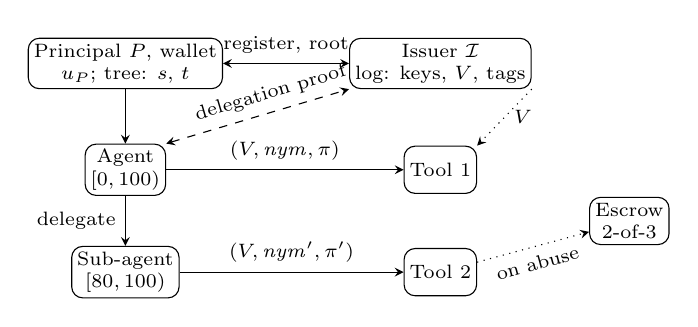
\begin{tikzpicture}[font=\scriptsize,>=stealth,box/.style={draw,rounded corners,align=center,minimum height=6mm,inner sep=2pt}]
\node[box] (P) at (0,2.3) {Principal $P$, wallet\\$u_P$; tree: $s$, $t$};
\node[box] (I) at (4.0,2.3) {Issuer $\mathcal{I}$\\log: keys, $V$, tags};
\node[box] (A) at (0,0.95) {Agent\\$[0,100)$};
\node[box] (S) at (0,-0.35) {Sub-agent\\$[80,100)$};
\node[box] (T1) at (4.0,0.95) {Tool 1};
\node[box] (T2) at (4.0,-0.35) {Tool 2};
\node[box] (E) at (6.4,0.3) {Escrow\\2-of-3};
\draw[<->] (P) -- node[above]{register, root} (I);
\draw[->] (P) -- (A);
\draw[->] (A) -- node[left]{delegate} (S);
\draw[<->,dashed] (A.north east) -- node[sloped,above,pos=0.6]{delegation proof} (I.south west);
\draw[->] (A) -- node[above]{$(V,\nym,\pi)$} (T1);
\draw[->] (S) -- node[above]{$(V,\nym',\pi')$} (T2);
\draw[->,dotted] (I.south east) -- node[right]{$V$} (T1.north east);
\draw[->,dotted] (T2) -- node[below,sloped]{on abuse} (E);
\end{tikzpicture}
\caption{Parties and the running example: the agent holds counters $[0,100)$ per tool and epoch and delegates $[80,100)$ to the hotel sub-agent. The issuer sees root requests and delegations, not presentations.}\label{fig:arch}
\end{figure}


\paragraph{Who runs the issuer, and why tools would accept the cost.} The anonymity set of a presentation is the set of principals of the same issuer whose mandates allow the same call in the same epoch against the same accumulator value. Every tool learns which issuer vouches for the caller. The scheme therefore helps only where one issuer serves many principals whom the tools must not tell apart. Three settings fit:
\begin{itemize}[leftmargin=*]
\item \emph{A platform or federation imposing data minimization on third-party tools.} An agent platform (or a federation of platforms) runs the issuer for all its users and requires tools that only need authorization (search, retrieval, read-only APIs, metered services) to accept presentations instead of user identities, as a contractual condition or to implement data protection by design (GDPR Art.~25). The anonymity set is then the platform's user base for that class and epoch.
\item \emph{A consortium of tools that do not need identity.} Tools that sell per-call access, such as data providers and inference endpoints, can accept the issuer's quota as proof of entitlement and lose nothing by not identifying callers.
\item \emph{A large organization towards external tools.} An enterprise issuer hides which employee or team calls an external tool. Here the tool learns the employer, and the anonymity set is bounded by the number of employees whose mandates allow the class. For a small organization this set may be too small to matter; the scheme then still hides the delegation structure and the call history, but not the organization.
\end{itemize}
Tools that legitimately need the user's identity (payment, delivery, booking under a name) gain nothing from \sys{} for their own calls, and Sec.~VII-D of the main paper shows that they let a coalition name the rest of the session. The running example of the main paper (travel booking with payment) is therefore the case where the scheme helps least: it protects the searches and the sub-agent's activity from tools that do not need the name, and it requires that identity-learning calls be made in a separate session, or at another time, from the rest of the task. E3 measures this: issuing the identity-learning call alone, at a random time within the next hour, cuts naming from 68\,\% to 22\,\% at 1{,}000 users against an attacker that matches amounts only within a short window. An attacker that joins the payment to the earlier quote of the same amount across the whole hour brings naming back to 44\,\% (its join is right 83\,\% of the time); when the decoupled call carries no value echoed from the task, for example a payment against an opaque order token that the search tool never saw, naming stays at 20\,\%. The design rule is therefore that a decoupled call must carry no amount, identifier or date that also appears in the task's other calls or results.

\paragraph{Operational cost for tools.} A tool verifies a presentation of \PresB{}~bytes in about \VerMs{}~ms of one core (the main paper's E1), against well under a millisecond for a JWT. It also keeps two pieces of state that must be shared by all its replicas: the single-use nonces it issued, and the seen-set of pseudonyms for the current epoch. Both are small and short-lived (one entry per call, dropped at the end of the epoch), and fit a shared key-value store with atomic insert (for example \texttt{SET NX} with a time-to-live of one epoch). The reservation of a pseudonym before verification (Sec.~IV of the main paper) makes concurrent verification by several replicas safe as long as the insert is atomic.

\paragraph{Relation to the MCP authorization specification.} Revision 2026-07-28 of the MCP specification requires, when authorization is used over HTTP, an OAuth bearer access token in the \texttt{Authorization} header of every request, issued for the server as audience (RFC~8707), and forbids servers to accept or transit other tokens~\cite{mcpauth}. Our binding carries the presentation in the request's \texttt{\_meta} field and is therefore \emph{outside} the core specification. Two deployment options are compatible with it:
\begin{itemize}[leftmargin=*]
\item \emph{As an authorization extension.} The specification defines optional, additive authorization extensions. A \sys{} extension would let a server advertise that it accepts presentations (with its tool descriptor) and define the \texttt{\_meta} field and the challenge request. Clients that do not implement it fall back to OAuth. In such an extension the nonce request would naturally be a dedicated JSON-RPC method or capability rather than a tool, so that clients unaware of the extension never show it to a model; the specification's extension repository (\texttt{modelcontextprotocol/ext-auth}) is where it would be proposed.
\item \emph{Together with a per-server domain token.} The client presents an ordinary bearer token issued by the domain's authorization server for this server (RFC~8707 audience, no user identity, shared by all principals of the domain), and the presentation in \texttt{\_meta} carries the per-call authorization. The access token then authenticates the domain, not the user; it is a bearer secret shared by many clients, so leaking it exposes only the OAuth layer, not the per-call authorization. If the authorization server issues a token per client instead, that token is a linking handle, and the deployment loses unlinkability towards the tool. We did not evaluate this option.
\end{itemize}
In our MCP binding the nonce request is a separate server operation (a \texttt{challenge} tool) that the client harness calls before each authorized call; it is not listed among the tools offered to the language model, so prompts are unchanged. It costs one extra round trip per call (E2 reports it).

\paragraph{Personal data and the escrow (GDPR).} The following is our reading, not legal advice.
\begin{itemize}[leftmargin=*]
\item \emph{Are presentations personal data for tools?} A presentation is pseudonymous data in the sense of Art.~4(5) GDPR: the escrow committee can attribute it with additional information that the tools do not hold. Under Recital~26 and the Court of Justice's relative approach in \emph{EDPS v SRB} (C-413/23~P, 4~September~2025)~\cite{cjeu2025srb}, and the EDPB's draft guidelines on pseudonymisation~\cite{edpb2025pseudo}, whether such data is personal for a given recipient depends on whether that recipient has means reasonably likely to be used to re-identify the person. A tool without access to the committee's keys may then not be processing personal data through the presentation itself. The call content and timing may still identify the person: E3 shows that a coalition pooling logs re-identifies many calls, so in realistic deployments the tools' logs remain personal data, and the issuer, which knows when delegations happen and which roots it issued, and the committee remain controllers or processors of personal data.
\item \emph{Roles.} The issuer and the platform that operates it determine the purposes and means of authorization and are controllers (jointly, Art.~26, if they decide together). The committee members act for the controller on documented instructions (processors, Art.~28) or as independent controllers if a law gives them their own task. Tools are controllers of the call content they receive.
\item \emph{Lawful basis for an opening.} An opening is a new processing operation and needs its own lawful basis under Art.~6, typically a legal obligation of the controller (Art.~6(1)(c)), which applies only where Union or Member State law compels the disclosure, for example a binding request from a competent authority (whose own processing then falls under Directive (EU) 2016/680), or a legitimate interest in investigating abuse that is not overridden by the principal's interests (Art.~6(1)(f)), assessed case by case.
\item \emph{Notification.} Informing the principal follows from the transparency duties (Arts.~13--14 and 15). It may be delayed or restricted where Union or Member State law allows it under Art.~23, for example during a criminal investigation.
\item \emph{Governance we recommend.} Three committee members independent of the platform and of each other; for every opening request, a log entry before any share is released, holding a commitment to the request and its justification that is opened once any investigation allows it (delayed transparency reconciles public accountability with the confidentiality of criminal investigations under Art.~23 GDPR and Directive (EU) 2016/680); and escrow keys scoped to a period and erased after the retention time, so that old ciphertexts become unopenable. Revocations are part of the scheme: the log accepts them only with an anonymous proof made with the revoked mandate's own credential (held by its holder and its parent) or with two committee signatures. These are design recommendations; the GDPR does not prescribe this committee.
\end{itemize}

\paragraph{Channels outside the cryptographic model.} Names or addresses in call arguments identify the principal (E3 measures how much content reveals). IP addresses and TLS sessions call for a relay such as Oblivious HTTP. The MCP session identifier and client information link the calls of one session; one stateless session per call removes this (E2). An OAuth access token per client identifies it; with \sys{}, tools need no client authentication beyond the presentation, or a token shared by the domain. The issuer sees when roots are issued (identified) and when delegations happen; wallets should reach it through a relay and not request roots right before use, and E3's issuer attacker assumes long-lived roots.

\paragraph{Revocation under a shared issuer (E4).} A presentation built against accumulator value $V$ and verified after a tool installed its successor is rejected when the grace window is zero. Two remedies were measured.
\begin{itemize}[leftmargin=*]
\item \emph{Wallet retry.} After a rejection, if the wallet has seen a newer value, it rebuilds the presentation once against that value, with the same counter and a fresh tool nonce. Reusing the counter is safe for the quota because tools release the reservation of a pseudonym whose proof fails, so a rejected pseudonym is never recorded. It has a privacy cost: the two attempts carry the same pseudonym, so a tool that rejects falsely can link them, and a counter released without a retry must not be reused for a later call to the same tool. Our wallet API enforces this: a released counter is stored with the hash of the call, reused only by the next presentation of the same call to the same tool in the same epoch, and burned otherwise. The unlinkability game does not model retries; for this reason the time-bounded window, not the retry, is the scheme's freshness mechanism (Sec.~IV of the main paper). A first variant that drew a new counter wasted quota (18 of 696 honest calls rejected) and was abandoned. Without either remedy, the scripted agent saw 80 of 460 honest calls rejected (17\,\%), as the LLM agents did, so the effect is not an artefact of the harness.
\item \emph{Time-bounded window.} The tool accepts the previous value only for $\Delta$ after its successor reaches the tool, which bounds the revocation delay by $\Delta$ plus propagation, whatever the revocation rate, and with batching at most two accumulator values coexist at a tool, so the anonymity set splits at most in two; a count-based window $W$ instead delays revocation by $W$ updates, which with sparse revocations means $W$ times their interval.
\end{itemize}
Both remedies avoid honest rejections only while revocations are published less often than a presentation takes to build and reach the tool (about 0.4--0.6~s here); an issuer guarantees this by batching revocations so that it publishes at most one value per $\Delta$. In our runs, new values were pushed to four tools over loopback (about 0.14~s) and the wallet shared the issuer's process, so the delays exclude propagation from the log to real tools and wallets. The scripted runs used a shared, niced login node (Intel Xeon Gold 6426Y), the LLM runs the H100 nodes (Table~\ref{tab:prov}).

\section{Additional evaluation results}\label{s:evalx}
This section gives the attack taxonomy (Table~\ref{tab:attacks}), the ablation of a presentation (Table~\ref{tab:ablation}), a summary of which mechanism fits which requirement (Table~\ref{tab:decide}), the cost of a presentation and of delegation versus the number of signed messages (Fig.~\ref{fig:costs}), the effect of the revocation list (Table~\ref{tab:rev}), the E3 results with their ranges over seeds (Table~\ref{tab:linkranges}), the provenance of every experiment (Table~\ref{tab:prov}), E4 success per configuration (Table~\ref{tab:e4cfg}), and the dependence of E3 naming on load (Fig.~\ref{fig:e3load}). All numbers are generated from the result files of the artifact, like those of the main paper.

\begin{table}[t]\centering\caption{Attack taxonomy: number of attacks per threat and the party that rejects them.}\label{tab:attacks}
\footnotesize\setlength{\tabcolsep}{3pt}
\begin{tabular}{@{}lrrrrrr@{}}\toprule Threat & $n$ & Prover & Issuer & Tool & Judge & Log\\\midrule
\inputtab tab_attacks.tex \end{tabular}\end{table}

\begin{figure}[t]\centering
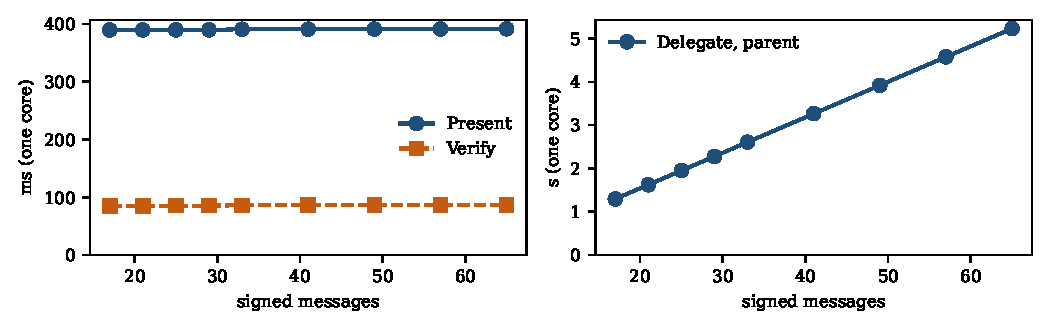
\includegraphics[width=0.9\textwidth]{fig_costs}
\caption{One server core. Left: presentation and verification time versus the number of signed messages. Right: delegation time for the parent; one range proof per action class.}\label{fig:costs}
\end{figure}

\begin{table}[t]\centering\caption{Revocation list size (medians, ms, one server core). Witness: issuer computes one witness; Batch: issuer revokes 100 more ids; Refresh: holder updates 5 witnesses.}\label{tab:rev}
\footnotesize\setlength{\tabcolsep}{3pt}
\begin{tabular}{@{}lrrrrr@{}}\toprule $|\mathcal{R}|$ & Witness & Batch & Refresh & Present & Verify\\\midrule
\inputtab tab_rev.tex \end{tabular}\end{table}

\begin{table}[t]\centering\caption{Ablation of a presentation (medians, ms, one server core).}\label{tab:ablation}
\footnotesize\setlength{\tabcolsep}{3pt}
\begin{tabular}{@{}lrrr@{}}\toprule Statements & Present & Verify & Bytes\\\midrule
\inputtab tab_ablation.tex \end{tabular}\end{table}

\begin{table}[t]\centering\caption{Which mechanism for which requirement.}\label{tab:decide}
\footnotesize\setlength{\tabcolsep}{3pt}
\begin{tabular}{@{}>{\raggedright\arraybackslash}p{0.5\textwidth}>{\raggedright\arraybackslash}p{0.35\textwidth}@{}}\toprule
Requirement & Mechanism\\\midrule
Authority and audit; linkability acceptable & JWT/Biscuit chain\\
Unlinkable by tools; issuer may see activity & batch one-time tokens\\
Unlinkable by tools and issuer; flat authority & blind tokens with PoP key\\
Abuse blocking without identification & anonymous blocklisting\\
Plus delegation, tree quota, subtree revocation, escrow & \sys{}\\\bottomrule
\end{tabular}
\end{table}

\begin{figure}[t]\centering
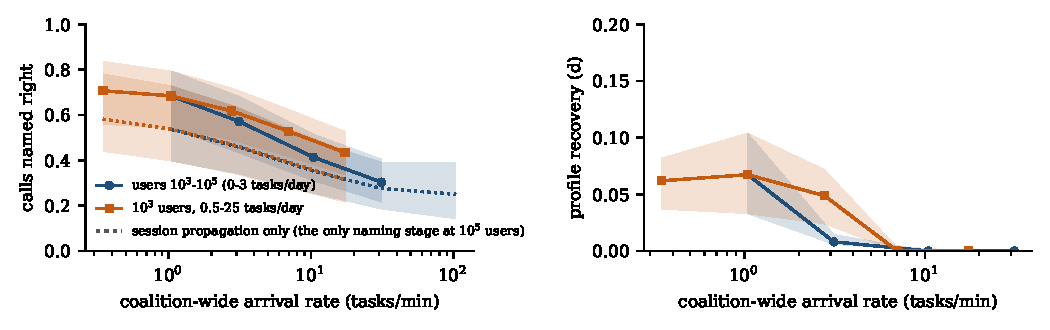
\includegraphics[width=0.95\textwidth]{fig_e3_load}
\caption{E3, \sys{} format, 5 seeds: naming of calls when one tool per task learns the identity, and profile recovery by attacker (d), against the task arrival rate across the coalition (tasks per minute, log scale), varied by population size and per-user task rate.}\label{fig:e3load}
\end{figure}

\begin{table}[t]\centering\caption{E3 collusion of 50 tools, \%, mean [min--max] over 5 seeds: profile recovery by attacker (d) and by the profile oracle at 1{,}000 users, (d) at 10{,}000 users, and naming of calls when one tool per task learns the user's identity, at 1{,}000 and 10{,}000 users.}\label{tab:linkranges}
\footnotesize\setlength{\tabcolsep}{3pt}
\begin{tabular}{@{}lrrrrr@{}}\toprule & \multicolumn{3}{c}{Profile recovery} & \multicolumn{2}{c}{Naming}\\ Token format & (d) & Oracle & (d), $10^4$ & $10^3$ & $10^4$\\\midrule
\inputtab tab_link_ranges.tex \end{tabular}\end{table}

\begin{table}[t]\centering\caption{Provenance of the experiments: code commit, build or harness hash (prefix of the SHA-256), platform and jobs. \texttt{results/SHA256SUMS-v2.2} lists the hashes of all result files. E1 ran on v2.2.0 (\texttt{96a694d}); a first run of campaign 1 (job 1680010) was uniformly slower on every operation and was excluded by a rule fixed before its rerun (all medians more than 10\,\% off the other campaigns) and rerun on another node; it is kept in \texttt{results/v22/zen/excluded\_node068}. E1 times the honest prove and verify paths only; the wallet's witness and spot checks add five pairing equations per refresh and two per published update. Commits after E4 v2.1 added checks outside those paths (class index, root layout, wallet checks) and a carving order that does not affect E4, whose delegations are one level deep. v2.2.1 changes only the log's revocation rule, which only the attack suite exercises.}\label{tab:prov}
\footnotesize\setlength{\tabcolsep}{3pt}
\begin{tabular}{@{}>{\raggedright\arraybackslash}p{0.17\textwidth}>{\raggedright\arraybackslash}p{0.2\textwidth}>{\raggedright\arraybackslash}p{0.24\textwidth}>{\raggedright\arraybackslash}p{0.3\textwidth}@{}}\toprule
Experiment & Commit & Build / harness & Platform, jobs\\\midrule
Attack suite & \texttt{cc54645} (v2.2.1) & \texttt{attacks} \texttt{163ed5ce} & Apple M5 Pro\\
E1 & \texttt{96a694d} (v2.2.0) & \texttt{bench} \texttt{a24a9cd0} (Zen), \texttt{08cd38c6} (laptop) & AMD EPYC 9534 (Zen), 3 exclusive nodes, 1 pinned core, jobs 1680015, 1680011, 1680012 (excluded: 1680010), multi-core 1680013; Apple M5 Pro\\
E2 & \texttt{02718067} (harness committed later) & \texttt{e2v21.py} \texttt{9a472e38} & Apple M5 Pro, 3 runs, load recorded\\
E3 & \texttt{dacd3b3}, \texttt{3266003}, \texttt{12bdc01} & \texttt{sim/e3v22.py} & Zen, jobs 1679921--1680000\\
E4 v2.1 & \texttt{060ced91} & mmpy \texttt{1ace11bf} & 1 H100 + Xeon Platinum 8462Y+ (Hedy), jobs 45427--45444, 48495, 48510\\
E4 v2.2, scripted & \texttt{e340685}, \texttt{a4149d7} & mmpy \texttt{c3c54fbe}, \texttt{0b120113} & Hedy login node (Xeon Gold 6426Y, shared, niced)\\
E4 v2.2, LLM & \texttt{a4149d7}, \texttt{df4f429} & mmpy \texttt{0b120113} & 1 H100 (Hedy), jobs 51013, 51014, 51052\\\bottomrule
\end{tabular}
\end{table}

\begin{table}[t]\centering\caption{E4, success on the honest templates (a, b, d) per configuration, \%, without authorization (none) and with \sys{} (MM): temperature 0 with tool latency (t0), its replication (t0\_rep), without tool latency (t0\_nolat), and temperature 0.7 over three seeds (t07).}\label{tab:e4cfg}
\footnotesize\setlength{\tabcolsep}{3pt}
\begin{tabular}{@{}lrrrrrrrr@{}}\toprule & \multicolumn{2}{c}{t0} & \multicolumn{2}{c}{t0\_rep} & \multicolumn{2}{c}{t0\_nolat} & \multicolumn{2}{c}{t07}\\ Model & none & MM & none & MM & none & MM & none & MM\\\midrule
\inputtab tab_e4_cfg.tex \end{tabular}\end{table}

\section{Evidence for Table 1}\label{s:table1}\sloppy
Partial (\(\circ\)) and inferred (\(^*\)) cells of Table~1 of the main paper, with the source of each; the artifact's \texttt{related-audit.md} quotes the passages.
\begin{itemize}[leftmargin=*]
\item Agentic JWT: delegation \(\circ\), a chained assertion names the downstream agent but specifies no narrowing of scope; binding \(\circ\), the token is scoped to an agent, intent and workflow step and a proof-of-possession key signs the HTTP request, without a nonce or request hash.
\item AP2 (v0.1.0): delegation \(\circ^*\), an intent mandate passes the user's authority to an agent, without multi-hop attenuation; binding \(\checkmark\), a cart mandate signs the specific purchase; traceable, mandates are shown to merchants.
\item DAC (mercurial): delegation \(\circ\), level-based only, attributes left to future work; escrow/trace \(\circ\), an opener exists but registration is anonymous.
\item UACS: delegation \(\circ^*\), the issuer updates hidden attributes under a proven relation, which can express attenuation; UACS does not claim delegation.
\item DAC from JWTs: delegation \(\circ^*\), each level discloses attributes selectively, which can express attenuation; offline \(\checkmark^*\), delegation needs no change to issuer infrastructure.
\item BBS per-verifier pseudonyms: unlinkable \(\circ\), only across verifiers; binding \(\circ^*\), a presentation header can carry a verifier challenge.
\item BBA+, Clone Wars, dynamic \(k\)-TAA, BLAC/SNARKBlock: escrow/trace \(\circ\), misuse (double spending, over-use, blocklisting) reveals or blocks the user, which is accountability, not escrow.
\item ACT, Privacy Pass, ARC: binding \(\circ\), the token binds a client message or the origin's challenge, not the call; Privacy Pass rate limit \(\circ\), rate-limited issuance is specified in an expired draft.
\item SD-JWT batch: unlinkable \(\circ\), only with one-time batch credentials, and the issuer can link; binding \(\circ\), the key-binding JWT binds a nonce, the audience and a hash of the disclosures, not the call.
\item Coconut: rate limit \(\circ\), a per-petition value prevents signing a petition twice.
\end{itemize}

\bibliographystyle{IEEEtran}
\bibliography{refs,refs2}
\end{document}
